\documentclass[conference]{IEEEtran}
\IEEEoverridecommandlockouts
% The preceding line is only needed to identify funding in the first footnote. If that is unneeded, please comment it out.
\usepackage{cite}
\usepackage{amsmath,amssymb,amsfonts}
\usepackage{algorithmic}
\usepackage{graphicx}
\usepackage{textcomp}
\usepackage{xcolor}
\def\BibTeX{{\rm B\kern-.05em{\sc i\kern-.025em b}\kern-.08em
    T\kern-.1667em\lower.7ex\hbox{E}\kern-.125emX}}
\begin{document}

\title{Deep Reinforcement Learning for Blackjack}

\author{
    \IEEEauthorblockN{Marius Oechslein}
    \IEEEauthorblockA{
        \textit{Faculty of Computer Science and Business Information Systems} \\
        \textit{University of Applied Sciences Würzburg-Schweinfurt}\\
        Würzburg, Germany \\
        marius.oechslein@study.thws.de
    }
}
\maketitle

% TODO: Main focus of paper:
% . Zuerst implementiere ich "traditional RL-methods" (Sarsa, Q-Learning, TD) als Baseline? 
% . Dann implementiere ich Deep Reinforcement Learning und versuche die Baseline zu erreichen.
% . Dann erhöhe ich den state-space durch das genaue counting aller Karten 
% . -> Hierbei möchte ich vergleichen, wie sich DQN im Vergleich zu traditionellen RL-Methoden verhält. 
% .		Ich habe 3 traditionelle, weil der Test dadurch allgemeingültiger ist und nicht von der Implementierungsdetails einer einzelnen Methode abhängt.


\begin{abstract}
In this study, we explore Blackjack using Reinforcement Learning. Specifically, we compare traditional Reinforcement Learning methods, namely Monte Carlo Control, SARSA, and Q-Learning, with the Deep Reinforcement Learning method called Deep Q-Learning.

Initially, all methods achieve the baseline objective of determining the optimal policy without card counting. Next, we introduce a simple card counting method, and all the approaches handle it effectively. Finally, we test the robustness of these methods by increasing the state-space from 11,000 to 1,024,000.

Remarkably, Deep Q-Learning performs well in this extensive state-space, while the traditional Reinforcement Learning methods struggle to estimate the value-function with the increased complexity.
\end{abstract}

\begin{IEEEkeywords}
	Blackjack, Monte Carlo Control, SARSA, Q-Learning, Deep Q-Learning
\end{IEEEkeywords}

\section{Introduction}
\subsection{Blackjack and Reinforcement Learning} 
Blackjack is a widely played card game in casinos worldwide. In 1962, mathematician Edward Thorp published a book outlining winning strategies for Blackjack \cite{b1}. This enabled players to gain an advantage over casinos in the game. However, subsequent rule changes by casinos have made it nearly impossible for players to win using those methods. Nevertheless, the game continues to intrigue mathematicians due to its probabilistic nature.

Thorp's groundbreaking idea was the introduction of card counting using the Complete Point Count System \cite{b1}. This simple method involves keeping a count that increases or decreases by +1 or -1 for each card seen during play, allowing players to keep track of the cards while playing.

\subsection{Reinforcement Learning for Blackjack}
The game can be represented as a Markov Decision Process, allowing the application of Reinforcement Learning techniques. The primary objective is to model Edward Thorp's basic strategy \cite{b1}.

All of the Reinforcement Learning methods play a large number of games while keeping track of a Q-Table containing the expected returns to each of the possible game states \cite{b4}.
While these methods are powerful, they require a substantial number of games to accurately model the Q-Table, especially as the game's state-space expands.

This study investigates the performance of Reinforcement Learning methods (Monte Carlo Control, SARSA, and Q-Learning) as we increase the state-space by modifying the card counting method. To make the card counting more complex, we keep track of the values of every observed card instead of a single counter, as in the case of the Complete Point Count System \cite{b1}.

\subsection{Deep Reinforcement Learning}
In 2013, DeepMind introduced a novel approach called Deep Reinforcement Learning, combining Deep Learning with Reinforcement Learning, as described in the paper "Playing Atari with Deep Reinforcement Learning" \cite{b2}. This method replaces the Q-Table with a deep neural network, enabling the estimation of value-functions for complex state-spaces that were previously challenging for traditional Reinforcement Learning methods.

In this study, we first explore whether Deep Reinforcement Learning can achieve the baseline performance of Edward Thorp's basic strategy and Complete Point Count System \cite{b1}. Additionally, we compare the performance of Deep Reinforcement Learning with more traditional RL-methods like Monte Carlo Control, SARSA, and Q-Learning, as the state-space expands.


\section{Methods}

\subsection{The Blackjack Environment}
In Blackjack, the game begins with the dealer and player each receiving two cards. The player can only see one of the dealer's cards and their own hand. The player has two options: take another card (Hitting) or not take another card (Standing). Although Blackjack has more options like Doubling Down and Splitting, this study focuses solely on Standing and Hitting. This decision was made to prioritize the Reinforcement Learning methods rather than the game's precise representation.

The player can choose to hit multiple times, aiming to get as close to a hand value of 21 as possible. After the player's turn, the dealer hits as long as their hand value is 16 or below. At the end of each game, the player's return is determined based on whether they win, lose, or draw. For Reinforcement Learning, the rewards are assigned as +1, -1, and 0.

To model the basic strategy using Reinforcement Learning, we consider one game as one episode. This is possible because the basic strategy relies solely on the dealer's card and the player's hand value, while the remaining deck information is irrelevant.

However, when introducing card counting, we need to extend one episode to multiple games. Card counting relies on information from previously played cards, in addition to the current game's cards. The ratio of high to low cards left in the deck affects the player's chances of winning. By extending one episode to play through a whole deck, the chances of encountering an imbalanced card deck increase, making card counting more relevant.

The Complete Point Count System \cite{b1} maintains a running score, which is updated every time the player sees a card:
\begin{itemize}
	\item +1 for: 2, 3, 4, 5, 6
	\item -1 for: 10, A
	\item 0 for: 7, 8, 9 
\end{itemize}
A high counting score benefits the player \cite{b1}, while a low counting score favors the dealer. This is because the dealer's chances of busting increase when there are more high cards than low cards remaining in the deck.

\subsection{State-action space}
To learn the basic strategy, we use a the state consisting of the player's hand value, the dealer's card value and whether the player has an usable ace. 
This makes a total number of 250 states that need to be considered:
\begin{itemize}
	\item 10 possible dealer states: 2,3,4,5,6,7,8,9,10,A
	\item 25 possible player states:
		\subitem No Ace: 4,5,6,7,8,9,10,11,12,13,14,15,16,17,18,19,20
		\subitem With Ace: 13,14,15,16,17,18,19,20
\end{itemize}

To incorporate the Complete Point Count System, the state must be extended by the counting score. The counting score can range from +24 (representing low six cards of each suit) to -20 (representing five high cards of each suit), which would result in a state-space of 11,000 states (250 states * (24 - 20)).

However, keeping track of every value of played cards significantly expands the state space to approximately 1,048,576,000 states (250 states * ($4^9$ number cards * (4 face cards * 4 states))) when playing through one card deck. Due to this immense state space, RAM problems occurred with the Google Colab Free version (12.7 GB RAM). Consequently, a simpler card counting method was adopted, which only tracks whether a card value has been played or not. This simplified approach still provides valuable information regarding the player's chances, particularly when indicating the presence of all four cards of a specific value remaining in the deck.

Using the advanced card counting method, the state space expands to 1,024,000 states (250 states * ($2^9$ * (4 face cards * 2 states))) when playing through one card deck.

This significant increase in state space provides an interesting opportunity to observe the performance of Deep Reinforcement Learning and compare it to other Reinforcement Learning methods.


\subsection{Reinforcement Learning methods}
All Reinforcement Learning methods follow a common approach of taking actions in an environment, observing the rewards, and keeping track of the expected rewards for each state-action \cite{b4}. Additionally, they all require a substantial number of episodes to accurately estimate the expected rewards \cite{b4}.

The main characteristics that distinguish different RL-methods are as follows \cite{b4}:
\begin{itemize}
	\item \textbf{On-policy vs. Off-policy Learning}: If the same policy is used for exploration and exploitation steps. 
	\item \textbf{Update Rule}: With what information the updates are done. 
	\item \textbf{Bootstrapping}: If updates are done based on prediction of future values. 
\end{itemize}

These are the terminologies used for the rest of this paper: 
\begin{itemize}
	\item Q: action-value function
	\item V: state-value function
	\item G: cumulative reward after visited state until the end of the episode 
	\item R: reward
	\item S: state
	\item A: action
	\item t: timestep
	\item $\gamma$: discount rate
	\item $\alpha$: learning rate
\end{itemize}

\subsubsection{Monte Carlo Control}
Monte Carlo Control (MC) was introduced in the book \textit{Reinforcement Learning: An Introduction} \cite{b4}. It is an on-policy learning method that employs the epsilon-greedy strategy to decide between exploration and exploitation. The update rule for Monte Carlo Control is as follows:
\begin{equation*}
	V(S_t) \leftarrow V(S_t) + \alpha [G_t - V(S_t)] \tag{1}
\end{equation*}
MC does not utilize Bootstrapping, meaning updates are solely based on real observations. Consequently, Monte Carlo Control converges at a slower pace compared to methods that employ Bootstrapping \cite{b4}.


\subsubsection{SARSA}
The State-Action-Reward-State-Action (SARSA) method, a member of the Temporal Difference Learning family, was also introduced in the book \textit{Reinforcement Learning: An Introduction} \cite{b4}. It belongs to the on-policy learning category, using the same policy for exploration and exploitation with the epsilon-greedy approach. In the update rule, SARSA takes the reward of the next state into consideration:
\begin{equation*}
	Q(S_t, A_t) \leftarrow Q(S_t, A_t) + \alpha [R_{t+1} + \gamma Q(S_{t+1}, A_{t+1}) - Q(S_t, A_t)] \tag{2}
\end{equation*}
This means that SARSA utilizes bootstrapping since $Q(S_{t+1})$ is used for updating $Q(S_t, A_t)$. 

\subsubsection{Q-Learning}
Q-learning, initially introduced by Watkins \cite{b5} and further discussed in \cite{b4}, is a Temporal Difference Learning method. It operates as an off-policy learning approach, employing bootstrapping \cite{b4}.
\begin{equation*}
	Q(S_t, A_t) \leftarrow Q(S_t, A_t) + \alpha [R_{t+1} + \gamma \max_a Q(S_{t+1}, a) - Q(S_t, A_t)] \tag{3}
\end{equation*}


\subsection{Deep Q-Learning}
Deep Q-Learning (DQN) was introduced in 2013 in the DeepMind paper \textit{Playing Atari with Deep Reinforcement Learning} \cite{b2}. The core idea of DQN involves replacing the Q-Table with a deep neural network \cite{b2}. Additionally, two crucial implementation components, an Experience Replay Buffer and a Target Neural Network, are presented in the following section.

The pseudo-code for DQN can be found in the \textit{Playing Atari with Deep Reinforcement Learning} paper \cite{b2}. For more details on the DQN architecture implementation, \textit{Implementing the Deep Q-Network} \cite{b6} serves as a helpful resource.


\subsubsection{Experience Replay Buffer} \label{replay-buffer}
During each step of the training loop, the Experience Replay Buffer is populated with the Experience of the current training step. An Experience comprises the following components: state, action, reward, and next state. For each training step, a random mini-batch is then sampled from the Buffer and used to train the neural network.

The Experience Buffer offers the advantage of reusing Experiences for neural network training, increasing data efficiency \cite{b2}. Additionally, sampling random mini-batches uniformly breaks the dependency between a state and its preceding state, aiding in the training of a more generalized neural network \cite{b2}.

The Buffer has a maximum size of 10,000. When this size is reached, the oldest Experiences are removed to make space for new Experiences.


\subsubsection{Target Neural Network}
In traditional Q-Learning \cite{b4}, the current Q-value is updated using the estimated Q-value of the next state. To achieve the same update rule in Deep Q-Learning, a target neural network, referred to as $Q^*$ in the DeepMind paper \cite{b2}, is utilized to predict the returns of the next state \cite{b6}. These predicted returns of the next state are then used for the loss function and gradient descent of the learning network \cite{b6}.

The target network starts with the same architecture as the learning neural network. However, the weights of the target neural network remain fixed and only get updated based on the weights of the training network. In the paper \cite{b6}, the weights are updated only every few training steps to lower training time. In the implementation for this paper, the weights are updated every training step, but with a update rate of only 0.005 to prevent overfitting.

Using the target neural network brings the advantages of more stable training and better-controlled estimation errors \cite{b6}.


\section{Experiments and Evaluation}
As an introductory note to the next section, the plots for the points of interest for the RL-methods Monte Carlo Control, SARSA, and Q-Learning were randomly chosen because they perform almost identically. The main noticeable difference among these methods is their training time. The results of these different methods are used interchangeably in this section to emphasize their similarities and suitability for modeling Blackjack.

Another reason for not displaying the plots of all methods is the sheer number of plots that would need to be shown.


\subsection{Basic Strategy}
Both the RL-methods and the Deep Q-Learning method closely approach Edward Thorp's baseline basic strategy \cite{b1}. For instance, Figure \ref{fig:monte-carlo-basic-strategy} closely resembles Edward Thorp's basic strategy for hitting and standing \cite{b1}. However, it is important to note that SARSA and Deep Q-Learning methods required significantly more training time to achieve this goal compared to Monte Carlo Control and Q-Learning. Although no exact training time comparison was conducted since the primary focus of this paper is on how the methods estimate with increasing state-space rather than their training time.

Furthermore, it is uncertain what specific rules Edward Thorp used for calculations in his book "Beat the Dealer" \cite{b1}. Hence, achieving the exact same basic strategy as Edward Thorp did \cite{b1} is unlikely. Nevertheless, the basic Blackjack rules used in this paper's implementation are likely similar to the rules employed by Edward Thorp.

\begin{figure}
	\centering
	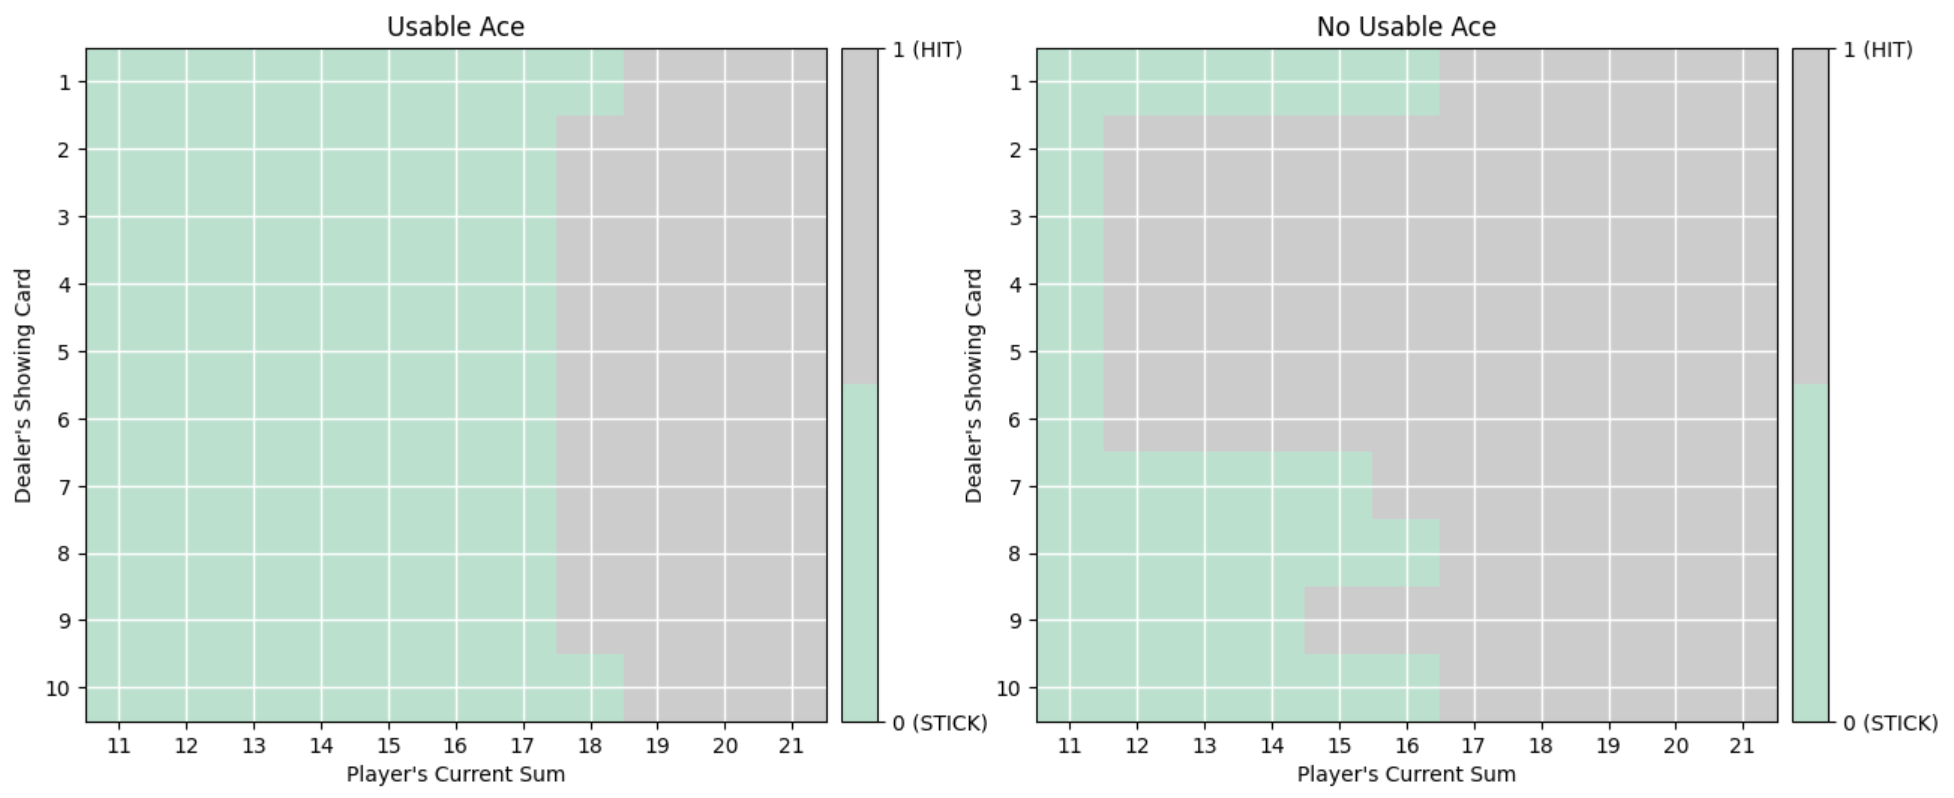
\includegraphics[width=70mm]{figures/MC/basic-100-million/policy.png}
	\caption{Monte Carlo Control policy after 100 million episodes. From own calculations.}
	\label{fig:monte-carlo-basic-strategy}
\end{figure}

In addition to the policy, the state-value function (shown in Figure \ref{fig:sarsa-state-value-basic}) closely resembles the state-value function of the basic strategy \cite{b4}. This suggests that the RL-methods can estimate the basic strategy effectively.

Please note that in Figure \ref{fig:sarsa-state-value-basic}, the dealer's ace is displayed on the right side of its states, whereas in \cite{b4}, the ace is shown on the left side.

\begin{figure}
	\centering
	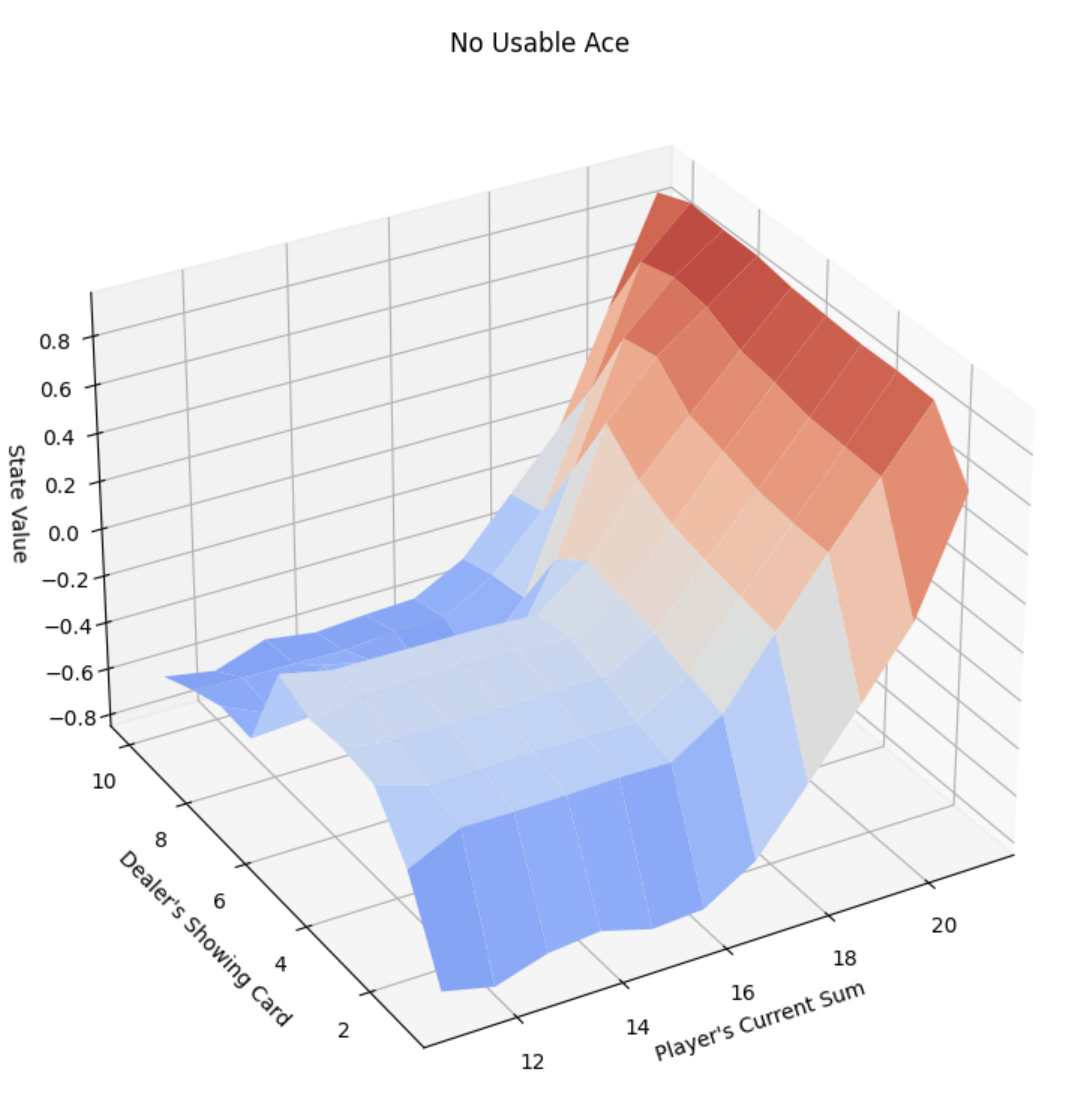
\includegraphics[width=70mm]{figures/MC/basic-100-million/value-function-no-usuable-ace.png}
	\caption{SARSA state-value function after 100 million episodes for case: no-usable ace. From own calculations.}
	\label{fig:sarsa-state-value-basic}
\end{figure}


\subsection{Complete Point Count Sytem}
For the Complete Point Count System, the main focus was to observe whether the player's policy adapts based on the counting score. A higher counting score indicates that there are more high cards than low cards left in the deck, as explained in the methods section. This boosts the player's winning chances since there is a higher probability of the dealer busting \cite{b1}. The player should therefore hit less in that case.

\begin{figure}
	\centering
	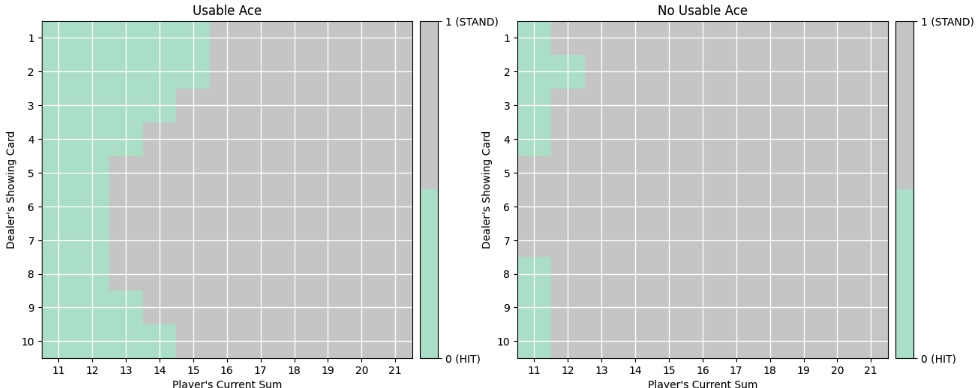
\includegraphics[width=70mm]{figures/DQN/counting-180000/policy-counting-7.png}
	\caption{DQN policy after 180 thousand episodes with a card counting score of 7. From own calculations.}
	\label{fig:dqn-card-counting-7}
\end{figure}

In this state, Figure \ref{fig:dqn-card-counting-7} suggests that the player should hit less frequently compared to the basic strategy shown in Figure \ref{fig:monte-carlo-basic-strategy}. This aligns with Edward Thorp's statement that a high ratio of high cards increases the player's winning probabilities by hitting less \cite{b1}.

For the case where the player has a usable ace, the policy in Figure \ref{fig:dqn-card-counting-7} remains mostly unchanged. This is reasonable since the ace's value can be reduced to 1 if the player's hand exceeds 21 after hitting a card. Consequently, hitting a card in this scenario only improves the player's winning chances, explaining why they should hit in that case.


\subsection{Increased state space - counting all cards}
For the following experiments the more advanced card counting method was employed, increasing the state-space to 1.027.000 states. 

\subsubsection{Monte Carlo Control, SARSA and Q-Learning}

\begin{figure}
	\centering
	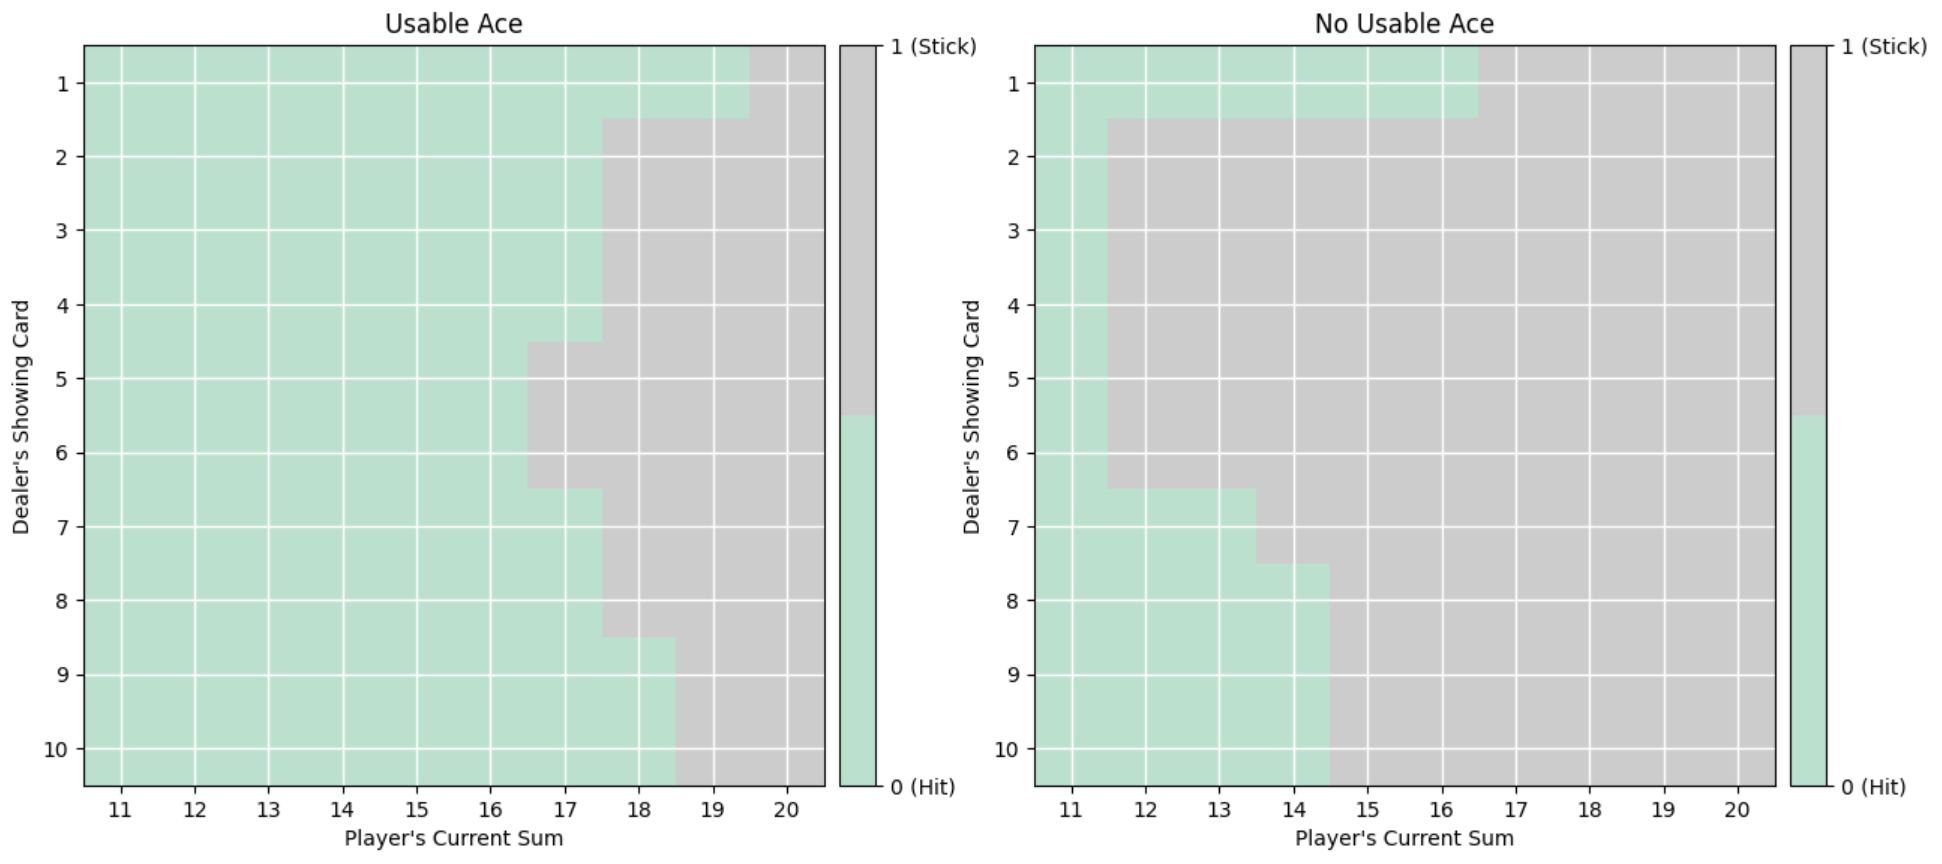
\includegraphics[width=70mm]{figures/Q-Learning/advanced-counting-10-million/policy-all-cards-played-1111111111.png}
	\caption{Q-Learning with advanced counting method. All cards have been played. From own calculations.}
	\label{fig:q-learning-advanced-all-cards-played}
\end{figure}

Figure \ref{fig:q-learning-advanced-all-cards-played} indicates that the policy for the state where all cards have been played at least once closely resembles the basic strategy from Figure \ref{fig:monte-carlo-basic-strategy}. It is crucial to recognize that this state is the most common and the ratio between high and low cards is even, and therefore, the policy should closely resemble the basic strategy \cite{b1}.

However, it is worth noting that the policy with this advanced counting method differs slightly from the basic strategy, which may be due to an insufficient number of games played in this state. Despite being the most common state, it is still uncertain to encounter this state in every episode.


\begin{figure}
	\centering
	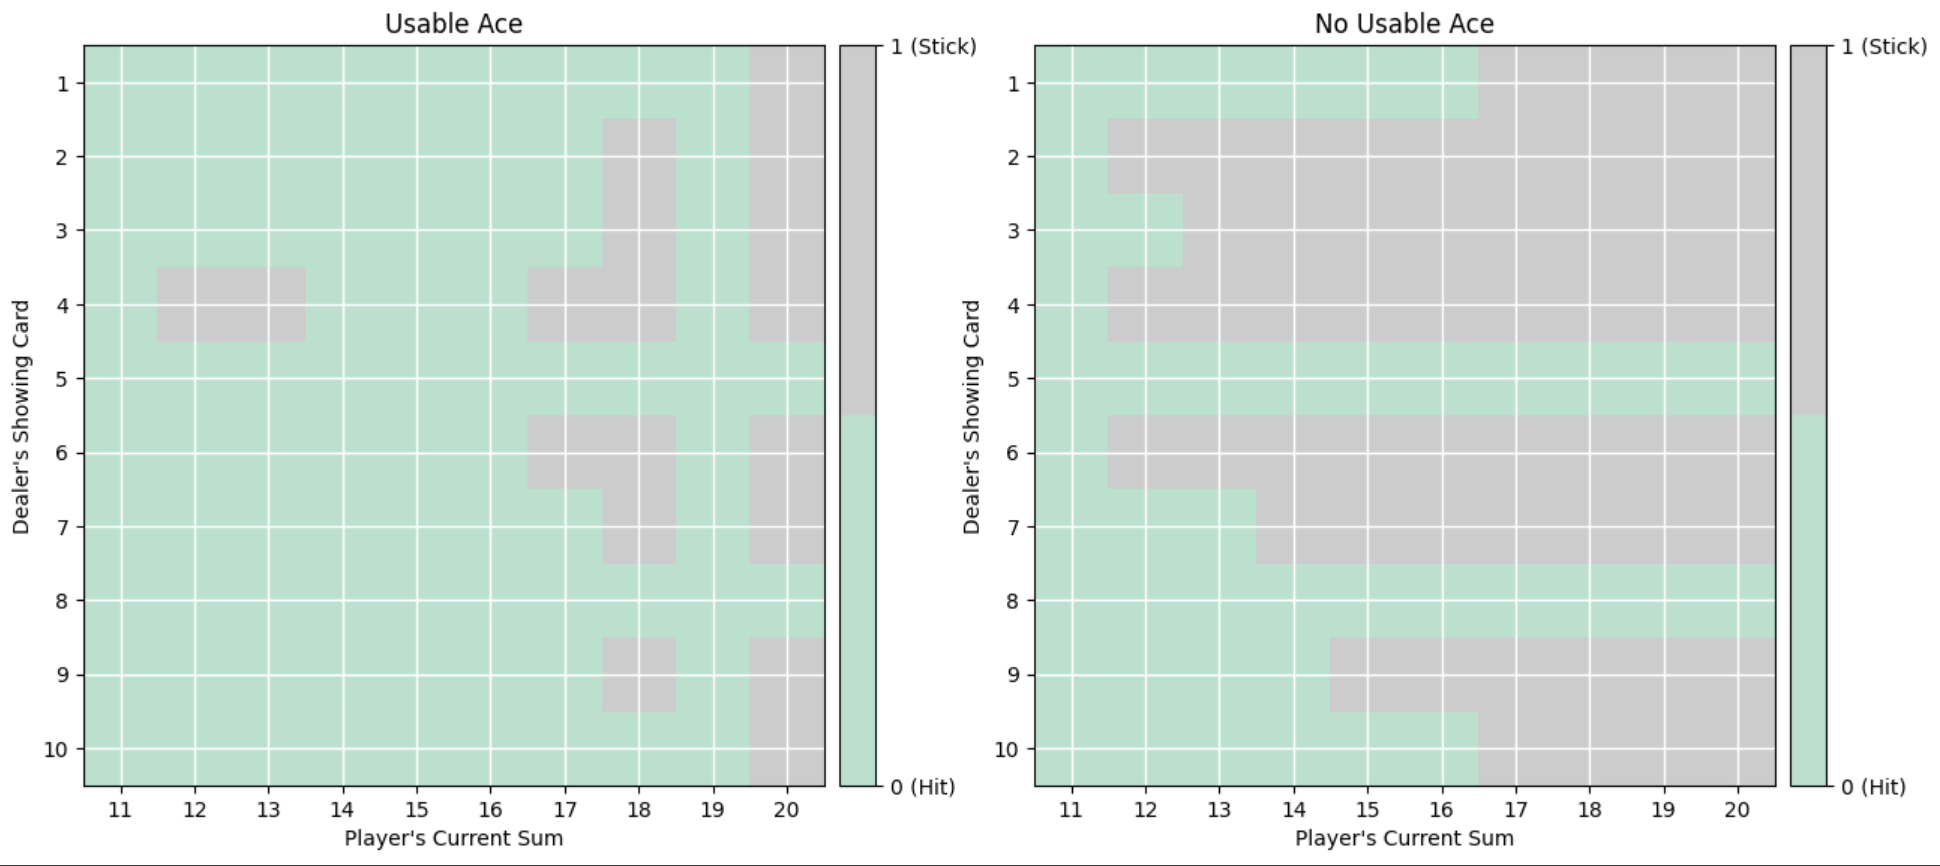
\includegraphics[width=70mm]{figures/Q-Learning/advanced-counting-10-million/policy-5-8-not-played.png}
	\caption{Q-Learning with advanced counting method. Only 5 and 8 have not been played. From own calculations.}
	\label{fig:q-learning-advanced-5-8-not-played}
\end{figure}

Figure \ref{fig:q-learning-advanced-5-8-not-played} for example shows the state where only the cards 5 and 8 have been played. This policy appears more noisy because this state is less likely compared to the state in Figure \ref{fig:q-learning-advanced-all-cards-played}. Consequently, there haven't been enough games played in this state for the RL-method to accurately estimate the policy.

\begin{figure}
	\centering
	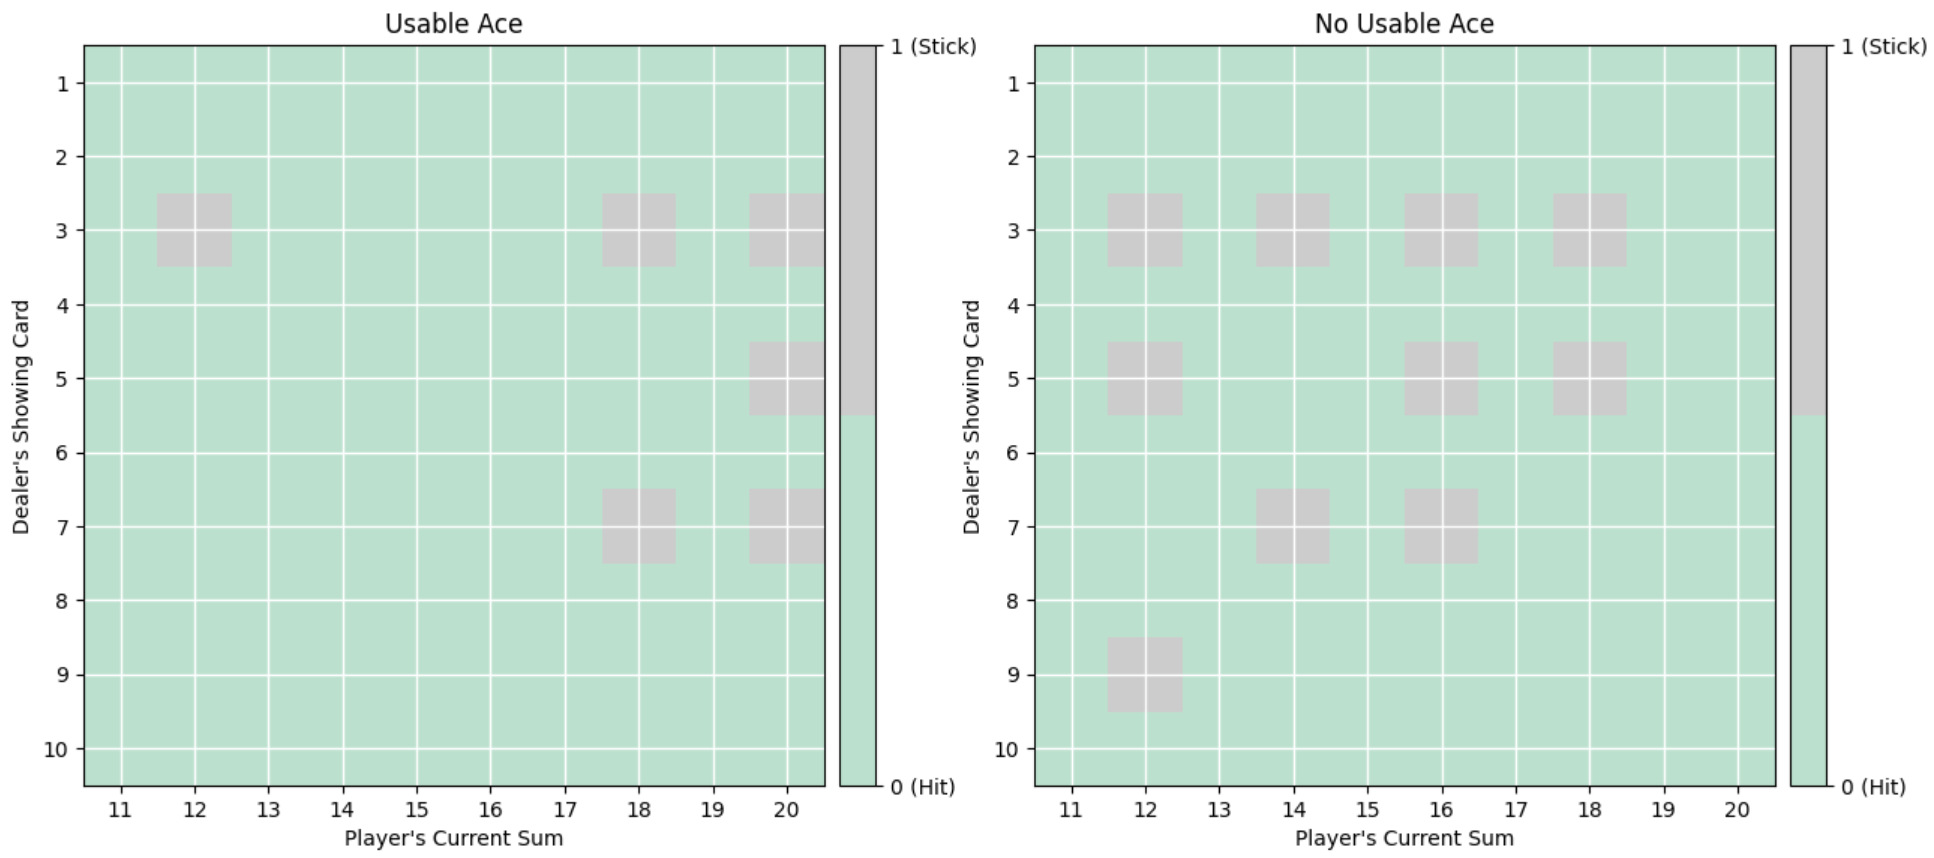
\includegraphics[width=70mm]{figures/Q-Learning/advanced-counting-10-million/policy-some-cards-played-1010101010.png}
	\caption{Q-Learning with advanced counting method. Every other card has been played, starting from Ace. From own calculations.}
	\label{fig:q-learning-advanced-every-other}
\end{figure}

Figure \ref{fig:q-learning-advanced-every-other} presents the policy for an even rarer state, leading to a very noisy policy. It is important to acknowledge that the value-function for all states is initialized with 0, and in this plot, zero is displayed as "Hit." This representation makes the policy appear less noisy in the plot than it actually is.


\subsubsection{Deep Q-Learning}
Regarding Deep Q-Learning, it's essential to note that each training iteration takes more time compared to the other discussed RL-methods due to training a neural network. Additionally, training a deep neural network requires a large number of training iterations. As a result, Deep Q-Learning takes longer to train. The training of the Deep Q-Networks was stopped after 180,000 training episodes due to the significant training time required. In contrast, the traditional RL-methods were trained on approximately 1,000 times more episodes compared to the Deep Q-Learning method, due to the difference in training time.

\begin{figure}
	\centering
	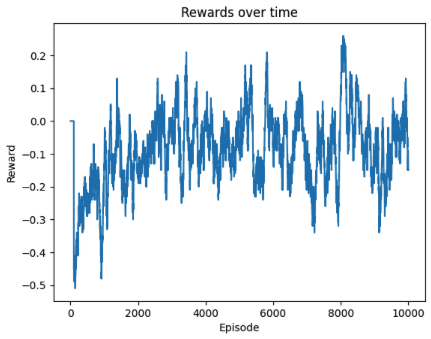
\includegraphics[width=70mm]{figures/DQN/rewards_over_time_10000.png}
	\caption{Deep Q-Learning with advanced counting method. Rewards over the first 10.000 episodes. From own calculations.}
	\label{fig:dqn-rewards-over-time}
\end{figure}

Figure \ref{fig:dqn-rewards-over-time} illustrates the DQN's learning progress during the first 10,000 episodes. Notably, the learning curve in the first 1,000 episodes is increases remarkably, given the complex state-space and neural network architecture. However, it's crucial to observe that the average reward stabilizes around -0.1 after this initial phase.

\begin{figure}
	\centering
	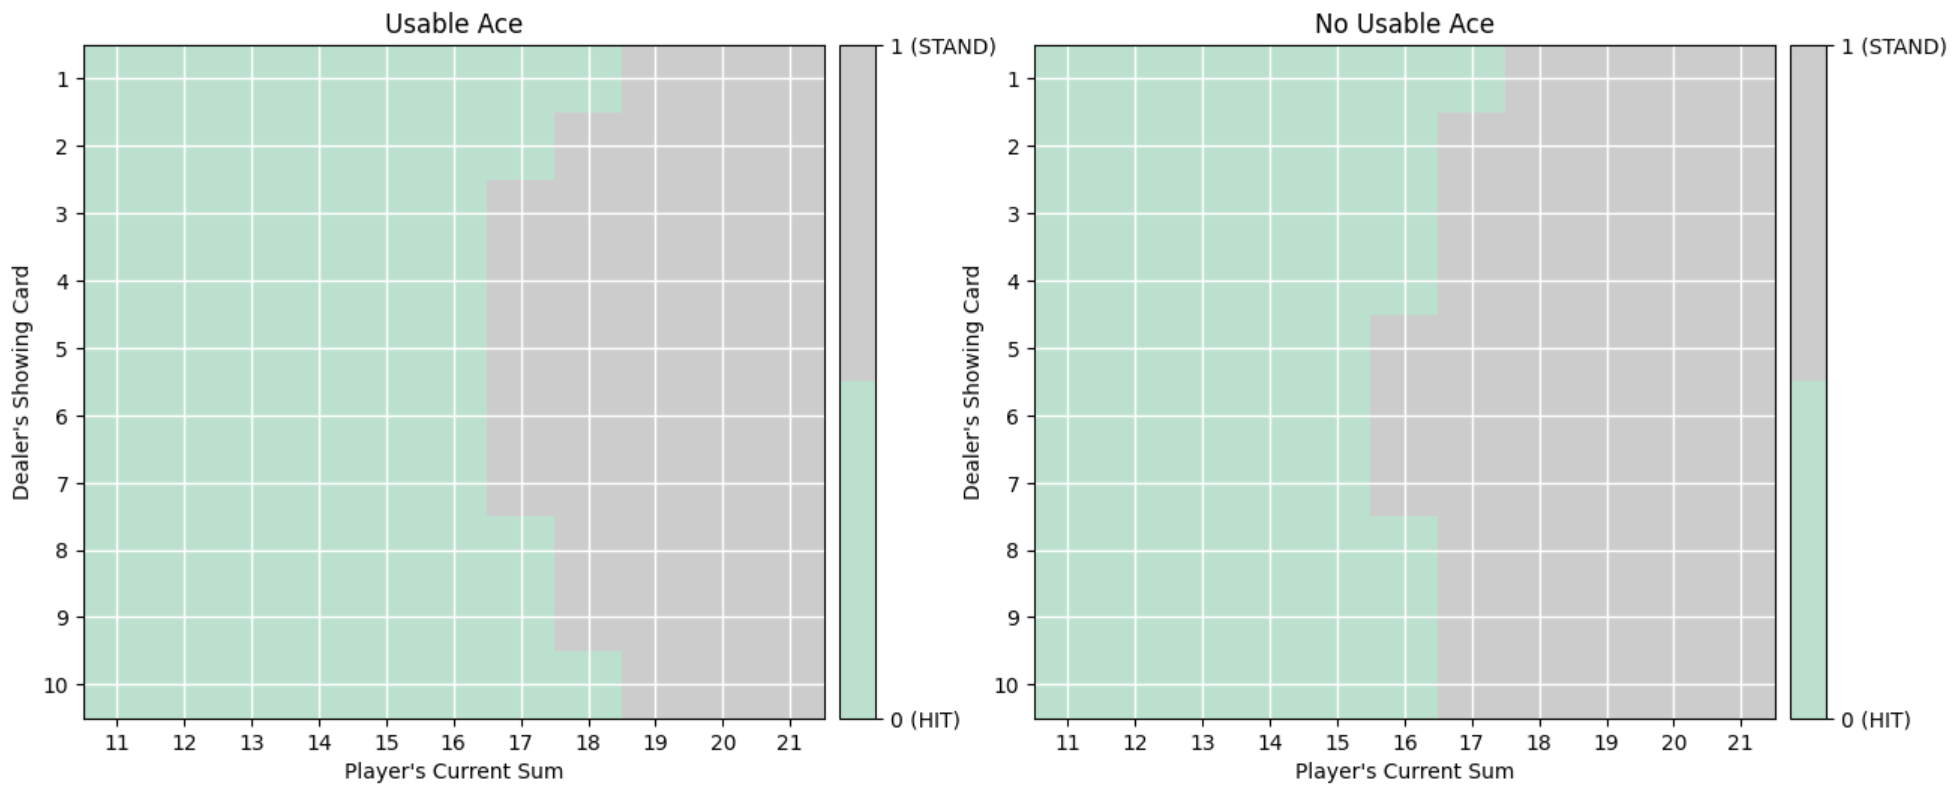
\includegraphics[width=70mm]{figures/DQN/advanced/policy-1010101010.png}
	\caption{Deep Q-Learning with advanced counting method. Every other card has been played, starting from Ace. From own calculations.}
	\label{fig:dqn-advanced-every-other}
\end{figure}

Figure \ref{fig:dqn-advanced-every-other} demonstrates that Deep Q-learning can approximate the policy effectively even for a rare state. It's worth noting that the same state was shown in Figure \ref{fig:q-learning-advanced-every-other} for Q-Learning, but Deep Q-Learning estimates the policy much better for this uncommon state compared to the RL-methods.

Notably the optimal policy for this uncommon state is unclear since it was not covered in \cite{b1} or \cite{b4}. This state involves an ace being played while a card with a value of 10 has not been played. Without further investigation, the perfect policy for this state is uncertain, given the unclear impact of these two card values. Nonetheless, the policy appears reasonable as it closely resembles the basic strategy \cite{b1}, which should logically apply to this similar state.

\begin{figure}
	\centering
	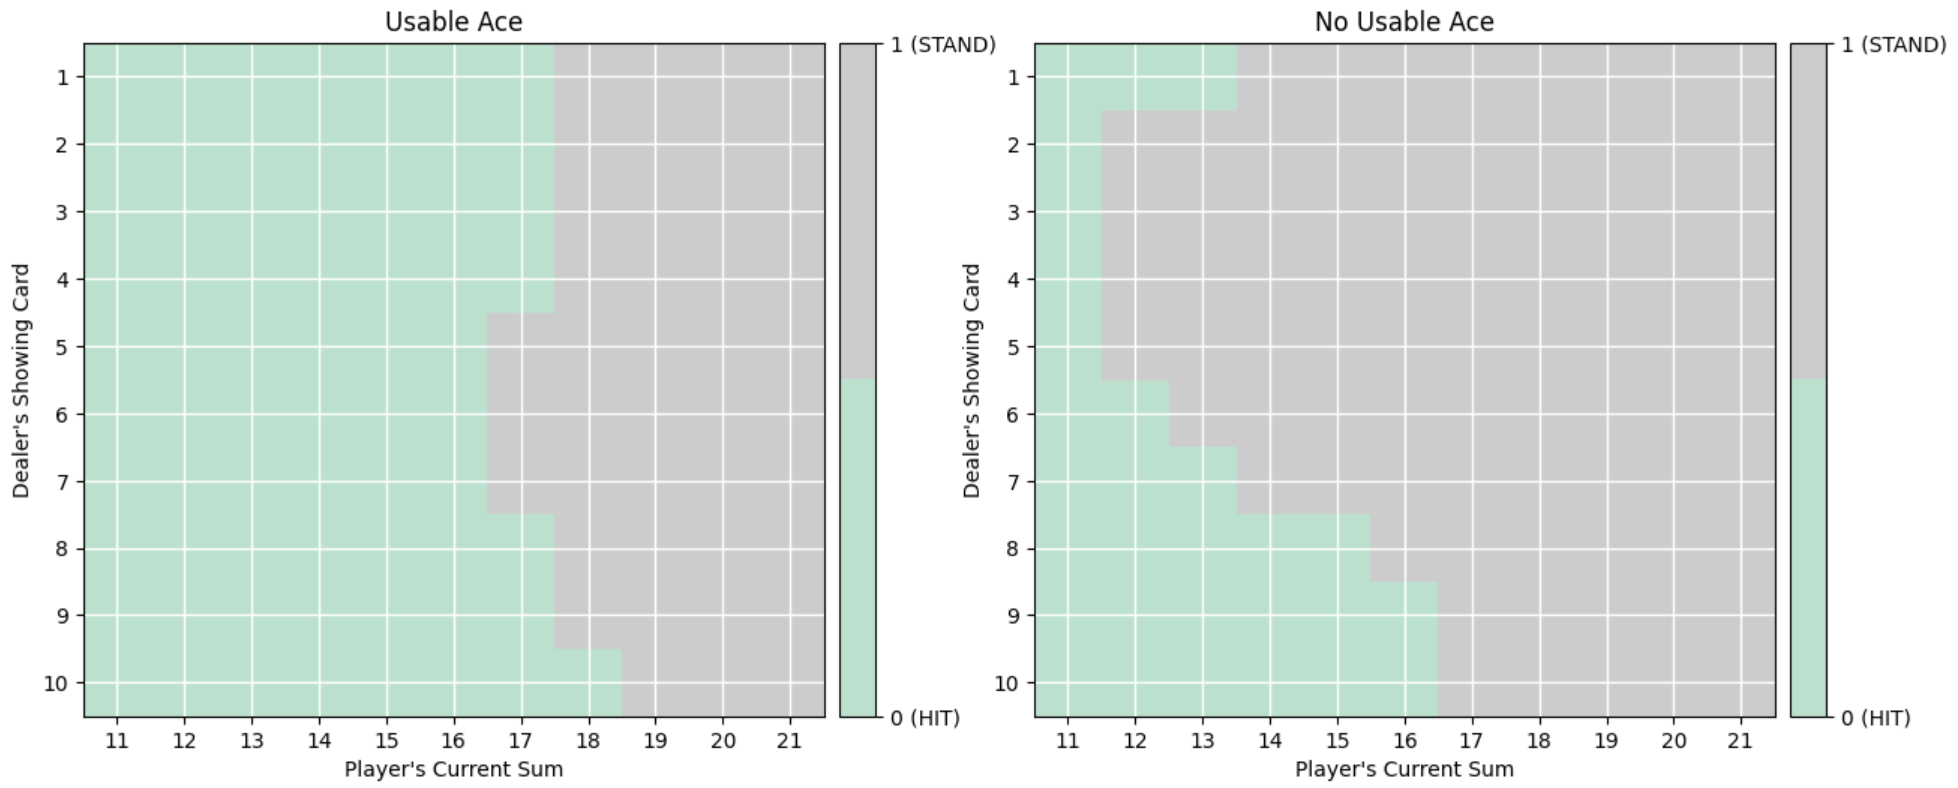
\includegraphics[width=70mm]{figures/DQN/advanced/policy-low-cards-played.png}
	\caption{Deep Q-Learning with advanced counting method. Only low cards (2,3,4,5,6) have been played. From own calculations.}
	\label{fig:dqn-advanced-only-low}
\end{figure}

Figure \ref{fig:dqn-advanced-only-low} displays the policy for the state where only low cards have been played, which closely resembles a high counting score for the Complete Point Count System in Figure \ref{fig:dqn-card-counting-7}. However, it is important to note that these two states are not equivalent because the advanced counting method does not track how many cards of a single value have been played.

% TODO: T-SNE plot?


\section{Conclusion}
In summary, both the RL-methods and the Deep Q-Learning method successfully modeled the baseline basic strategy from \textit{Beat the Dealer} \cite{b1}.

When the state-space was expanded to 1,024,000 states, the traditional RL-methods (Monte Carlo Control, SARSA, and Q-Learning) faced challenges in estimating the optimal policy. In contrast, Deep Q-Learning performed remarkably well, accurately estimating the optimal policy even for very uncommon states.

Further study the following four areas would be interesting:

First, it is noteworthy that the training of the DQN was stopped after 180.000 episodes. Interestingly between 120.000 and 180.000 training episodes, the estimated policy improved noticably and further training of the DQN could therefore yield more insights. 

Secondly, the desired advanced counting method, which keeps track of every played card-value, could not be examined due to hardware limitations. Testing this method with better hardware could provide valuable insights into a optimal strategy for all game states.

Evaluating the performance of the DQN when removing its two implementation details - the Experience Replay Buffer and Target Neural Network - would be interesting. Although DeepMind suggests less robust training \cite{b2}, scientific benchmarks for this scenario are currently lacking, to my knowledge.

Lastly, testing the trained DQN without further training on other similar card games would be intriguing. This idea is inspired by the \textit{Playing Atari with Deep Reinforcement Learning} paper, where the trained model achieved super-human performance in different Atari games without additional training \cite{b2}.


\begin{thebibliography}{00}
\bibitem{b1} Thorp, E. O. (1966). Beat the dealer: A winning strategy for the game of twenty-one (Vol. 310). Vintage.
\bibitem{b2} Mnih, V., Kavukcuoglu, K., Silver, D., Graves, A., Antonoglou, I., Wierstra, D., \& Riedmiller, M. (2013). Playing atari with deep reinforcement learning. arXiv preprint arXiv:1312.5602.
\bibitem{b3} Mnih, V., Kavukcuoglu, K., Silver, D., Rusu, A. A., Veness, J., Bellemare, M. G., ... \& Hassabis, D. (2015). Human-level control through deep reinforcement learning. nature, 518(7540), 529-533.
\bibitem{b4} Sutton, R. S., \& Barto, A. G. (2018). Reinforcement learning: An introduction. MIT press.
\bibitem{b5} Watkins, C. J., \& Dayan, P. (1992). Q-learning. Machine learning, 8, 279-292.
\bibitem{b6} Roderick, M., MacGlashan, J., \& Tellex, S. (2017). Implementing the deep q-network. arXiv preprint arXiv:1711.07478.
\end{thebibliography}
\end{document}
